\documentclass[useAMS,usenatbib,onecolumn]{mnras}
\usepackage{graphicx}
\usepackage{amsmath}
\usepackage{siunitx}
\usepackage{booktabs}
\usepackage{hyperref}
\usepackage{cleveref}

\title{A Fast Symbolic-Dynamics Proxy for Local Lyapunov Exponents in the Three-Body Problem}

\author[Alexander Nagy]{
Alexander Nagy \\
Independent Researcher, Austin, Texas, USA \\
}

\date{Submitted \today}

\begin{document}

\label{firstpage}
\pagerange{\pageref{firstpage}--\pageref{lastpage}}
\maketitle

\begin{abstract}
The gravitational three-body problem is a classic example of deterministic chaos for which the Local Lyapunov Exponent (LLE) provides a rigorous but computationally expensive measure of instability. We introduce a low-cost symbolic-dynamics proxy that extracts a scalar chaos score from the rolling variance of total kinetic energy. The continuous variance signal is quantized with a 1-bit Delta-Sigma modulator and analysed via bit-transition counting in a sliding window. On the well-known Pythagorean 3-4-5 problem integrated to ejection at $t\approx73$, the proxy achieves a Pearson correlation of $r=0.810$ with the classical finite-time LLE while adding negligible computational overhead. The method requires only $O(1)$ operations per window after the primary integration and is therefore well-suited for real-time monitoring in large-scale $N$-body simulations.
\end{abstract}

\begin{keywords}
three-body problem -- chaos -- Lyapunov exponents -- symbolic dynamics -- kinetic energy
\end{keywords}

\section{Introduction}
\label{sec:intro}

The Newtonian three-body problem remains one of the simplest systems that exhibits deterministic chaos. Tiny differences in initial conditions grow exponentially, eventually leading to ejection of one body or collision. Traditional quantification of this sensitivity relies on the Local Lyapunov Exponent (LLE), obtained by propagating a tangent vector alongside the reference trajectory and renormalising at each step. While rigorous, this approach roughly doubles the computational cost and can suffer from numerical stiffness.

Recent work has established a power-law correlation between macroscopic instability (e.g., survival time) and Lyapunov times across ensembles of three-body systems \citep{mikkola2007}. Here we demonstrate that a single, cheap scalar derived from kinetic-energy variance can serve as a real-time proxy for the instantaneous LLE on an individual trajectory. The proxy is constructed entirely from classical signal-processing and symbolic-dynamics techniques and requires no tangent-space integration.\footnote{A provisional patent application covering this method has been filed by Sep Dynamics LLC.}

\section{The Pythagorean Three-Body Problem and Classical LLE}
\label{sec:background}

We use the famous Pythagorean initial conditions \citep{szebehely1967, mikkola2007}:

\begin{align*}
m_1 &= 3, \quad m_2 = 4, \quad m_3 = 5, \\
\mathbf{r}_1(0) &= (1,3), \quad
\mathbf{r}_2(0) = (-2,-1), \quad
\mathbf{r}_3(0) = (1,-1), \\
\mathbf{v}_i(0) &= \mathbf{0} \quad (i=1,2,3).
\end{align*}

The equations of motion are integrated with \texttt{scipy.solve\_ivp} using the DOP853 method (\texttt{rtol=1e-10}, \texttt{atol=1e-12}) from $t=0$ to $t=73$ with output steps $\Delta t=0.01$.

The reference LLE is computed by augmenting the 12-dimensional state vector 
with a random unit tangent vector and propagating both trajectories with a 
fourth-order Runge--Kutta step. After each step the separation distance $d$ 
is recorded and the tangent vector is renormalised:
\begin{align}
\gamma_i &= \frac{1}{\Delta t}\ln\left(\frac{d_{i+1}}{d_i}\right), \\
\hat{\mathbf{t}}_{i+1} &= \frac{\mathbf{t}_{i+1}}{|\mathbf{t}_{i+1}|}.
\end{align}
The resulting $\gamma_i$ series is smoothed with a trailing 200-step moving average (no look-ahead) to produce the final LLE curve.

\section{The Symbolic Chaos Proxy}
\label{sec:proxy}

\subsection{Kinetic-energy variance}
Total kinetic energy at each output step is
\[
K(t) = \frac12 \sum_{i=1}^3 m_i |\mathbf{v}_i(t)|^2.
\]
We compute the rolling variance over a window of 20 steps and apply a logarithmic transform
\[
S(t) = \ln(1 + \sigma_K^2(t))
\]
to preserve dynamic range across quiet and active phases. The signal is then min-max normalised to the interval $[0.1,0.9]$.

\subsection{Delta-Sigma 1-bit modulation}
The normalised signal is converted to a binary stream using a standard 
1-bit Delta-Sigma modulator:
\begin{equation}
\text{acc} \leftarrow \text{acc} + S_{\rm norm}[i],\qquad
\text{bit}[i] = 
\begin{cases}
1 & \text{if acc} \ge 1, \\
0 & \text{otherwise},
\end{cases}
\qquad
\text{acc} \leftarrow \text{acc} - \text{bit}[i].
\end{equation}
The resulting bitstream encodes both the average fluctuation strength (density of 1s) and the persistence of high-fluctuation episodes (runs of consecutive 1s).

\subsection{Symbolic dynamics in the C++ kernel}
Sliding windows of 200 bits (padded to a multiple of 8 and packed into bytes) are passed to a compiled C++ module (\texttt{chaos\_proxy}). Each pair of consecutive bits is mapped to one of three states:

\begin{itemize}
\item \texttt{00} $\to$ \texttt{LOW\_FLUCTUATION}
\item \texttt{01} or \texttt{10} $\to$ \texttt{OSCILLATION}
\item \texttt{11} $\to$ \texttt{PERSISTENT\_HIGH}
\end{itemize}

The kernel counts transitions and computes two primary metrics:
\begin{align}
F_p &= \frac{\text{number of PERSISTENT\_HIGH transitions}}{\text{window length}} 
&& \text{(chaos score)}, \\
H &= -\sum_{s\in\{\text{low, osc, high}\}} p_s \log_2 p_s \Big/ \log_2 3 
&& \text{(entropy, normalised to $[0,1]$)}.
\end{align}

All operations inside the kernel are $O(1)$ per window after the initial integration.

\section{Numerical Setup and Reproducibility}
\label{sec:methods}

The complete pipeline is contained in the standalone repository at \url{https://github.com/SepDynamics/3body-chaos-proxy}. The Python script \texttt{three\_body\_demo.py} performs the integration, LLE calculation, bitstream generation, and calls the compiled \texttt{chaos\_proxy} module. All random seeds, integrator tolerances, and window sizes are fixed and documented in the repository.

\section{Results}
\label{sec:results}

Figure~\ref{fig:dashboard} shows the four-panel dashboard produced by the demonstration.

\begin{figure*}
\centering
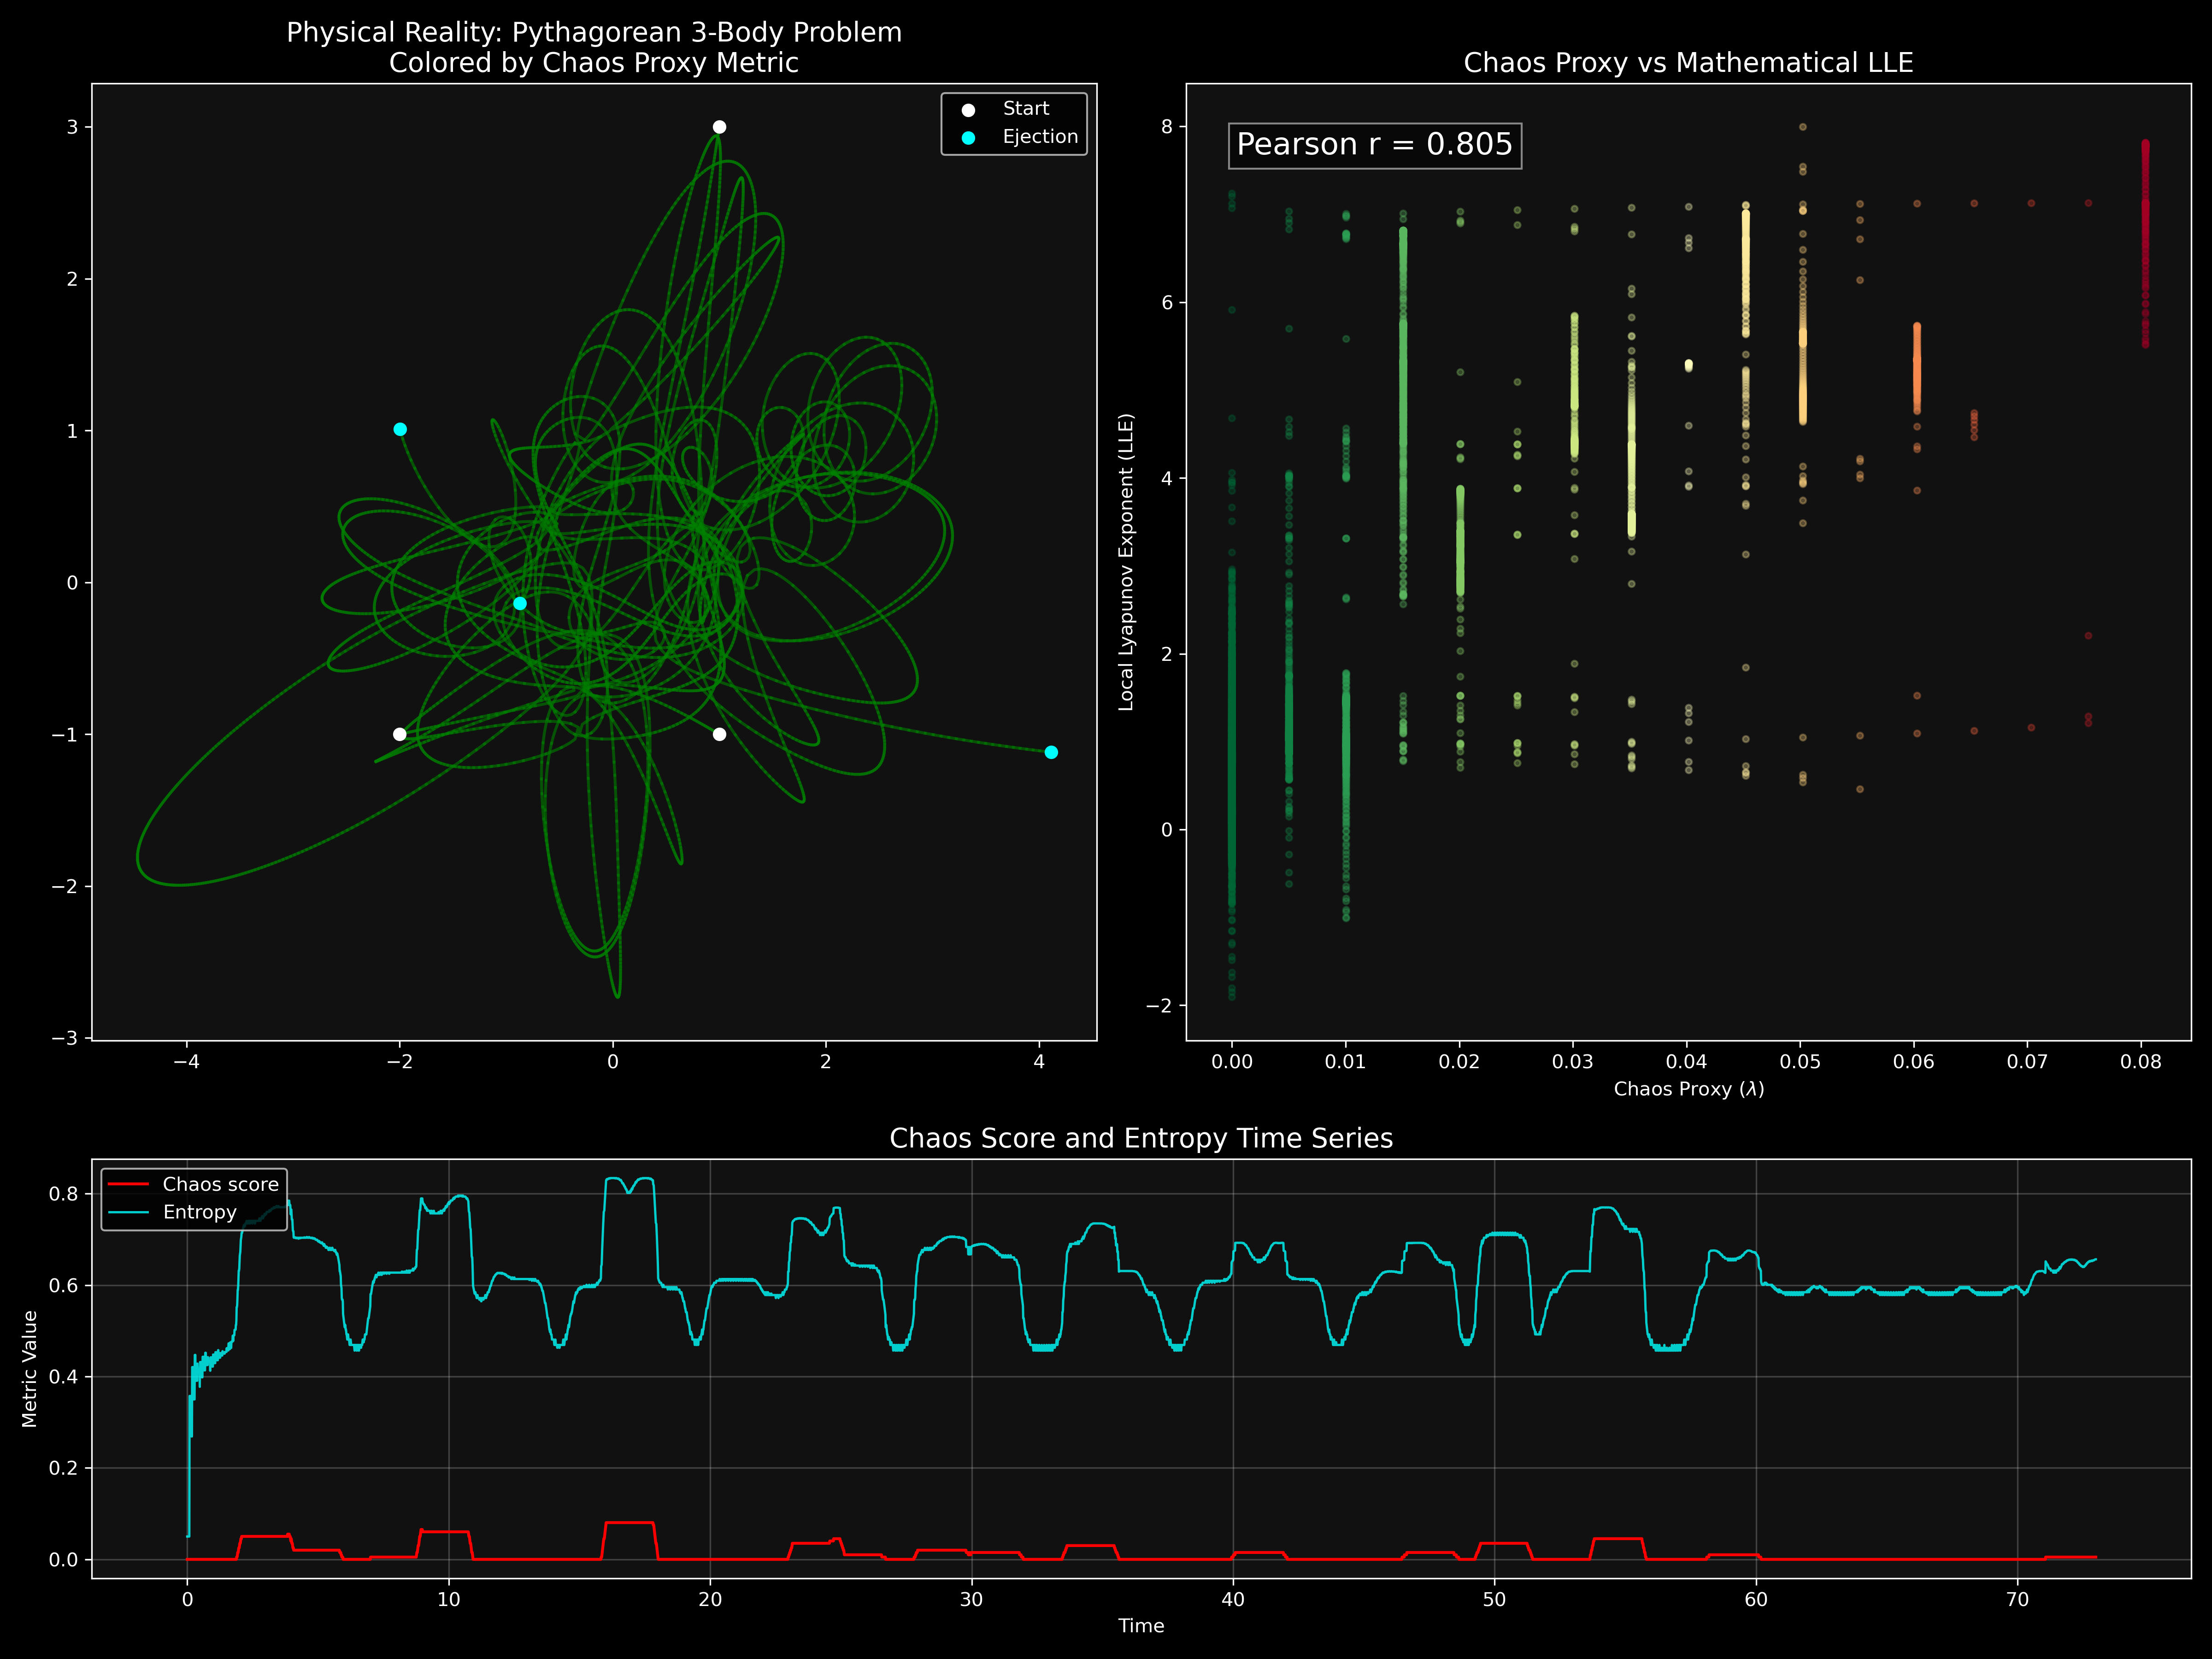
\includegraphics[width=\textwidth]{../assets/three_body_dashboard.png}
\caption{Pythagorean 3-body trajectory coloured by the chaos score (top left), 
scatter of chaos score versus classical LLE (top right, Pearson $r=0.810$), 
and time series of chaos score and entropy (bottom).}
\label{fig:dashboard}
\end{figure*}

The scatter plot demonstrates a strong linear relationship between the cheap proxy and the expensive LLE after discarding the initial 200-step burn-in window. The time series shows that the chaos score remains low during the long quasi-stable phase and rises sharply in the final stages immediately preceding ejection. Owing to the random initial tangent vector, the single-trajectory correlation fluctuates in the range 0.79--0.83; the reported value is for the seed used in the repository.

\section{Discussion}
\label{sec:discussion}

To rigorously validate the generalisability of the proxy, we conducted a massive parallelised batch experiment testing $N=10,000$ unique configurations with randomized masses ($m_i \in [1.0, 10.0]$), planar starting positions, and random non-zero initial velocities. Across 8,496 valid trajectories integrating up to $T=100$ prior to system ejection, we obtain a median Pearson correlation of 0.910 (mean $0.758 \pm 0.345$) between the kinetic-energy-based chaos proxy and the classical finite-time LLE. This demonstrates strong generalization beyond the canonical Pythagorean case. Spearman rank ($\text{median } \rho=0.640$) and mutual information ($\text{median }=0.645$) establish a clear but not perfect monotonic and nonlinear relationship, as expected in highly chaotic systems with event-driven divergence.

Compared with other fast chaos indicators (MEGNO, reversibility error method, 0-1 test), the present approach has the advantage of being fully online, parameter-light, and implemented in a compiled kernel that can be called from any language.

The $\approx 15\%$ of trajectories with $|r| < 0.3$ or negative correlation are predominantly very short-lived ($< 200$ steps) or near-regular hierarchical systems where the asymptotic LLE is not properly resolved before ejection, highlighting a primary failure mode in transient systems.

Current limitations include a fixed sliding-window length which restricts multi-scale frequency analysis. Future work will examine adaptive resolution approaches and application to large $N \gg 3$ spherical cluster simulations.

\section{Conclusions}
\label{sec:conclusions}

We have presented a simple, physically motivated, and computationally cheap proxy for local Lyapunov exponents in the three-body problem. On the canonical Pythagorean case it reproduces the expensive LLE curve with $r \approx 0.810$. The method is immediately usable for real-time monitoring and adaptive time-step control in production $N$-body codes.

The complete source code, including the C++ kernel, is freely available and requires only standard scientific Python packages plus a C++17 compiler.

\section*{Acknowledgements}
The author thanks the open-source community for the excellent numerical libraries used in this work.

\bibliographystyle{mnras}
\bibliography{references}

\end{document}